


%\subsection{La ricerca a Padova: l'esperimento RFX}

\subsection{fusione termonucleare}

La fusione termonucleare controllata nasce dall'idea di favorire la
possibilità che due nuclei di atomi leggeri si trovino ad una distanza
inferiore alla barriera columbiana così da permetterne la
trasformazione in unico nucleo di massa superiore. L'avvicinamento
necessario a realizzare questo processo si ottiene per collisione dovuta
ad un'indotta forte agitazione termica (modello classico), a cui
statisticamente si aggiunge un contributo dovuto all'effetto tunnel
(modello quantomeccanico).

Il difetto di massa tra reagenti e prodotti di fusione, e quindi la
quantità di energia liberata, è tanto più marcato quanto maggiore è la
differenza di energia di legame per nucleone rispetto alla variazione di
numero atomico. Ecco perchè risulta vantaggioso utilizzare isotopi di
atomi a basso numero atomico: essi presentano contemporaneamente una
bassa forza columbiana di repulsione, una maggiore energia cinetica
rispetto all'atomo non caricato, è un'alta differenza di energia di
legame. 

Tipicamente le reazioni studiate sono di quattro tipi:


\begin{align}
 \deuterio + \deuterio & \quad \rightarrow \quad  \elio3 + \neutrone + 3.3MeV \\
 \deuterio + \deuterio & \quad \rightarrow \quad  \trizio + \protone + 4.0MeV \\
 \deuterio + \elio3    & \quad \rightarrow \quad  \elio4 + \protone + 18.4MeV \\
 \deuterio + \trizio   & \quad \rightarrow \quad  \elio4 + \neutrone + 17.6MeV
 \label{eq:D-T}
\end{align}

Ognuna possiede una caratteristica sezione d'urto da cui si evince che
la reazione a più alta probabilità è la \eqref{eq:D-T} tra Deuterio e
Trizio\footnote{Trizio prodotto di fissione del Litio ...}. Essa avviene
a valori di energia non inferiori a $5keV$ e raggiunge il massimo di
efficenza a $15keV$. In questa situazione i reagenti si trovano allo
stato di plasma: un gas completamente ionizzato quasi elettricamente
neutro di dimensioni superiori alla lunghezza di Debye
$\lambda_{De}$. A causa dell'alta temperatura non esiste materiale in
grado di contenere la reazione senza inevitabilmente inquinarla.

Una soluzione a questo problema, studiata da oltre 60 anni, è
rappresentata dalle macchine a confinamento magnetico, in cui il
``contenitore'' del plasma è costituito da un gradiente di campo in una
camera a vuoto generalmente toroidale\footnote{un'altro metodo studiato
è l'ICF in cui il confinamento è ottenuto attraverso l'implosione di un
guscio sferico contenente la miscela D-T che viene compressa da raggi
laser o fasci di ioni ad alta energia}.

In siffatto sistema l'obiettivo è quello di soddisfare il cd ``criterio
di Lawson'', ossia di raggiungere uno stato di funzionamento tale per
cui il tasso di reazione sia sufficiente ad autosostenere l'energia
spesa per mantenere il plasma ignito.  La ricerca di un simile risultato
influenza sicuramente la scelta del modello di studio: ad esempio, si
potrebbe ipotizzare di costruire esperimenti di fusione attraverso
acceleratori di particelle, ma la netta predominanza della sezione
d'urto di ionizzazione rispetto alla fusione porterebbe ad un dispendio
di energia di vari ordini di grandezza maggiore rispetto a quella
ricavabile dalla reazione\footnote{ad esempio per una lastra di trizio
colpita da ioni di deuterio si ha: $\sigma_{ion} \approx 10^7
\sigma_{DT}$ quindi per ottenere i 17MeV della fusione sarebbe
necessario un consumo di $10^7$MeV.}.

La progettazione strutturale di ogni macchina da fusione rispecchia la
disposizione scelta per il campo interno. Sono state proposte molteplici
soluzioni geometriche lineari (come la ``bottiglia magnetica'') e
toroidali; quest'ultime sono apparse da subito topologicamente più
vantaggiose, in quanto il toro rappresenta l'unica superficie compatta
connessa orientabile su cui sia possibile definire un campo vettoriale
continuo senza punti critici\footnote{ovvero: definito un campo
vettoriale sulla superficie, non vi è alcun punto in cui esso si
annulli, caratteristica che permette alle linee di campo di ricombinarsi
su se stesse minimizzando l'energia spesa e massimizzando la stabilità
del plasma.}.

Considerando dei parametri specifici per la perdita di energia, come ad
 esempio perdite di frenamento (bremsstrahlung radiation) o di
 collisione (collisional and turbolent phenomena), si può riassumere
 l'efficenza della macchina attraverso un singolo valore detto ``triplo
 prodotto''\cite{cecco}:

\begin{equation}
 n \tau_E T_i \geq 3 \cdot 10^{21} m^{-3}s \cdot keV
\end{equation}

Contemporaneamente si può dimostrare che la curva di ignizione del
plasma che soddisfa il criterio di Lawson mostra un minimo a $T_i \simeq
20keV$; tale valore è la temperatura che si cerca di ottenere nel
bilancio del triplo prodotto variando densità ($n$) e tempo di
confinamento ($\tau_E$).


Per tutte le istallazioni a confinamento elettromagnetico, le
configurazioni del campo consistono in un inseme di componenti
magnetiche toroidali e poloidali; a seconda delle loro caratteristiche,
si dividono in tre principali categorie:
\begin{itemize}
\item{Tokamak}, in cui sono presenti entrambi i campi, ma con netta
     prevalenza di quello toroidale, che ha sostanzialmente la funzione
     di stabilizzare perturbazioni veloci.
\item{RFP} un elaborazione dello \emph{z-pinch}\footnote{vedi infra pg
     xxx} stabilizzato o \emph{screw-pinch}, in cui la componente
     toroidale è equiparabile a quella poloidale al punto da avere
     valore invertito al bordo (da cui il nome, ``reversed field
     pinch''); a questa condizione è affidato il raggiungimento di uno
     stato quiescente del plasma. Rispetto alla configurazione Tokamak
     la stabilità è più critica, ma l'efficenza del sistema è ampiamente
     superiore.
\item{Stellarator} in cui la geometria del campo è costruita disponendo una
     complessa struttura di bobine che favoriscono l'avvitamento della
     colonna di plasma.
\end{itemize}



\subsection{esperimento RFX e configurazioni RFP}


A Padova la ricerca sulla fusione ha condotto negli anni alla
realizzazione della macchina RFX basata sul modello RFP.  

%%%%%%%%%%%%%%%%%%%%%%%%%%%%%FIGURA%%%%%%%%%%%%%%%%%%%%%%%%%%%%%%%%%%%%%
\begin{figure}[ht]
 \centering
 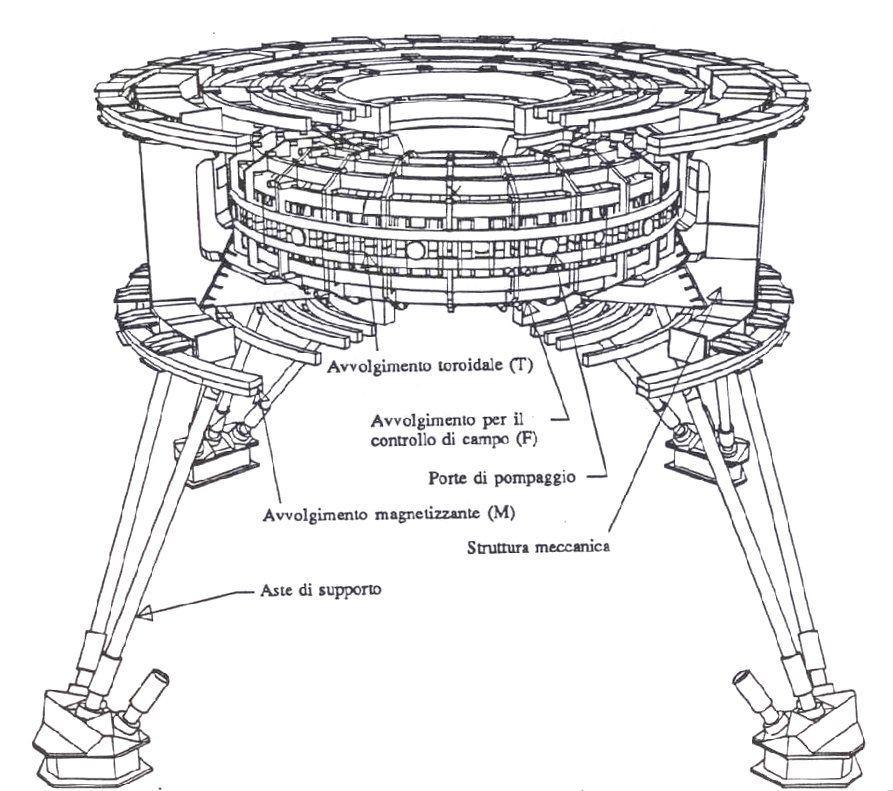
\includegraphics[ width=8cm ] {images/rfx2.jpg}
 \caption{Vista prospettica dell'esperimento RFX}
\end{figure}
%%%%%%%%%%%%%%%%%%%%%%%%%%%%%FIGURA%%%%%%%%%%%%%%%%%%%%%%%%%%%%%%%%%%%%%

La scarica per un sistema \emph{z-pinch} stabilizzato, dove $\Btor \sim
\Bpol$ si origina creando un campo toroidale con le bobine del solenoide
toroidale; attraverso una variazione del flusso concatenato con il toro
si induce poi nel gas una tensione toroidale e quindi, attraverso il
processo di ionizzazione, una corrente $I_p$ che cresce fino a
raggiungere il valore finale voluto. Man mano che la corrente di plasma
sale, si genera un campo poloidale che contribuisce, con la tensione
delle linee e la pressione magnetica, a determinare la situazione di
equilibrio radiale finale. La colonna di plasma quindi viene compressa e
ciò diventa significativo quando i due campi hanno all'incirca la stessa
intensità al bordo: infatti la pressione cinetica del plasma è molto
bassa e la pressione magnetica gioca un ruolo decisivo nella strizione.
Il plasma compresso concentra infatti il campo toroidale e crea nella
zona esterna una regione di quasi vuoto con un plasma tenue a bassa
conducibilità. Si osservano i seguenti profili per $\Btor , \Bpol ,q$.

%%%%%%%%%%%%%%%%%%%%%%%%%%%%%FIGURA%%%%%%%%%%%%%%%%%%%%%%%%%%%%%%%%%%%%%
\begin{figure}[ht]
 \centering
  \subfigure[z-pinch stabilizzato]{ \includegraphics[ width=4cm ]
  {images/profili-zp.png} } 
  \subfigure[reversedfield pinch]{ \includegraphics[ width=4cm ]
  {images/profili-RFP.png} }
  \caption{Profili di $B_\phi$ $B_\theta$ e $q$ rispetto alla posizione dall'asse del toro}
\end{figure}
%%%%%%%%%%%%%%%%%%%%%%%%%%%%%%%%%%%%%%%%%%%%%%%%%%%%%%%%%%%%%%%%%%%%%%

Tale configurazione presenta un minimo nell'andamento del fattore di
sicurezza che comporta uno Shear nullo. Il criterio di Suidam non è
soddisfatto e le superfici adiacenti il punto minimo risuonano
concatenando le linee di campo e innescando una perturbazione instabile.
L'unica soluzione a questo problema è un ribaltamento di $\Btor$ in modo
da rendere monotono l'andamento di $q$:

I primi zeta-pinch stabilizzati entrarono in funzione nei primi anni '60
in particolare il più rilevante fu ZETA con dimensioni simili a quelle
di RFX. I risultati, giudicati sul momento, furono mediocri: la macchina
presentava un regime turbolento, cui talvolta seguiva una fase
quiescente, un fenomeno a quel tempo di difficile spiegazione.

Il primo modello teorico fu proposto da Taylor nel 1974 \cite{taylor}:
egli ipotizzò, e dimostò, che la fase quiescente di ZETA corrispondeva
al passaggio ad una configurazione RFP tramite autorovesciamento del
campo toroidale poiche tale stato doveva corrispondere ad un minimo
energetico.

\begin{comment}
L'imposizione di Taylor fu che, contemporaneamente al minimo energetico,
fosse soddisfatta su tutto il volume di plasma la condizione detta di
``elicità'', ovvero:

\begin{equation}
K_0 = \int_{V_0}\vettore{A} \cdot \vettore{B} dV
\label{eq:elicità}
\end{equation}

mentre l'energia del plasma è considerata trascurando la pressione che
quindi è di natura essenzialmente magnetica:

\begin{equation}
W = \int_V \frac{B^2}{2\mu_0} dV
\end{equation}

La minimizzazione effettuata attraverso moltiplicatore di Lagrange 

\begin{equation}
 \delta(W+ \mu K_0) = 0
\end{equation}

risulta nella relazione:

\begin{equation}
\nabla \times \vettore{B} = \mu \vettore{B}
\label{eq:vincolo_taylor}
\end{equation}

da cui ricordando l'equazione di Maxwell 
$\nabla \times \vettore{B} =\mu_0 \vettore{J}$ 
si ottiene il valore del moltiplicatore:

\begin{equation}
 \mu = \mu_0 \frac{\vettore{J} \cdot \vettore{B} }{B^2} = \mu_0 \frac{J}{B}
\end{equation}

Tale relazione unitamente alla condizione di ``force free equilibrium''
( $\vettore{J}\times\vettore{B} = 0$ ) è stata calcolata nella
approssimazione cilindrica dallo stesso Taylor, e conduce ad una
soluzione dell'andamento di campo descritto tramite funzioni di
Bessel:

\begin{align}
& \Btor = B_0 J_0 (\mu r) \\
& \Bpol = B_0 J_1 (\mu r) \\
& B_r = 0
\end{align}


ricordando il valore di primo zero per la funzione di bessel $J_0$ si
trova che per avere rovesciamento la parete va posta ad una distanza
tale che $\mu a > 2.405$ che confrontato con la \eqref{eq:vincolo_taylor}
porge un valore per il parametro di pinch
\begin{equation}
 \Theta = \frac{\Bpol (a)}{\langle \Btor \rangle} = \frac{\mu a}{2} > \frac{2.405}{2} 
\end{equation}

[finire]
\end{comment}
 






